\documentclass{article}

\usepackage{hyperref}
\hypersetup{
    colorlinks=true,
    linkcolor=blue,
    filecolor=magenta,      
    urlcolor=cyan,
}

% for including notebooks
\usepackage{pdfpages}

\usepackage{fancyhdr}
\usepackage{extramarks}
\usepackage{amsmath}
\usepackage{amsthm}
\usepackage{amsfonts}
\usepackage{tikz}
\usepackage{float}
\usepackage[plain]{algorithm}
\usepackage{algpseudocode}
\usepackage{caption}
\usepackage{subcaption}

\usepackage{listings}
\usepackage{color} 
\definecolor{mygreen}{RGB}{28,172,0} 
\definecolor{mylilas}{RGB}{170,55,241}

\lstset{
    basicstyle=\scriptsize\sffamily\color{black},
    frame=single,
    numbers=left,
    showspaces=false,
    showstringspaces=false,
    tabsize=1
}
\lstset{language=Matlab,%
    %basicstyle=\color{red},
    breaklines=true,%
    morekeywords={matlab2tikz},
    keywordstyle=\color{blue},%
    morekeywords=[2]{1}, keywordstyle=[2]{\color{black}},
    identifierstyle=\color{black},%
    stringstyle=\color{mylilas},
    commentstyle=\color{mygreen},%
    showstringspaces=false,%without this there will be a symbol in the places where there is a space
    numbers=left,%
    numberstyle={\tiny \color{black}},% size of the numbers
    numbersep=9pt, % this defines how far the numbers are from the text
    emph=[1]{for,end,break},emphstyle=[1]\color{red}, %some words to emphasise
    %emph=[2]{word1,word2}, emphstyle=[2]{style},    
}

\topmargin=-0.45in
\evensidemargin=0in
\oddsidemargin=0in
\textwidth=6.5in
\textheight=9.0in
\headsep=0.25in


\linespread{1.1}

\pagestyle{fancy}
\fancyhf{}
\lhead{\hmwkAuthorName}
\chead{\hmwkClass: \hmwkTitle}
\rhead{\leftmark}
\lfoot{\lastxmark}
\cfoot{\thepage}

\renewcommand\headrulewidth{0.4pt}
\renewcommand\footrulewidth{0.4pt}

\setlength\parindent{0pt}

\newcommand{\hmwkTitle}{Assignment \ 1}
\newcommand{\hmwkDueDate}{February 14, 2020}
\newcommand{\hmwkClass}{Control Theory}
\newcommand{\hmwkClassInstructor}{Mike Ivanov}
\newcommand{\hmwkAuthorName}{\textbf{Artem Bakhanov (B18-03)}}

%
% Title Page
%

\title{
    \vspace{2in}
    \textmd{\textbf{\hmwkClass:\ \hmwkTitle}}\\
    \normalsize\vspace{0.1in}\small{Due\ on\ \hmwkDueDate\ at 11:59pm}\\
    \vspace{0.1in}\large{\textit{\hmwkClassInstructor\ }}
    \vspace{3in}
}

\author{\hmwkAuthorName}
\date{}

\begin{document}

\maketitle

\pagebreak

\tableofcontents

\pagebreak

\section{Introduction}
    I created a GitHub repository \href{https://github.com/artembakhanov/ControlTheoryHomework}{here}.
    All the problems are solved by me, Artem Bakhanov, a student of Innopolis University. My variant is \textbf{g}.
    
\section{Problem 2 (TF)}
\begin{figure}[ht]
        \centering
        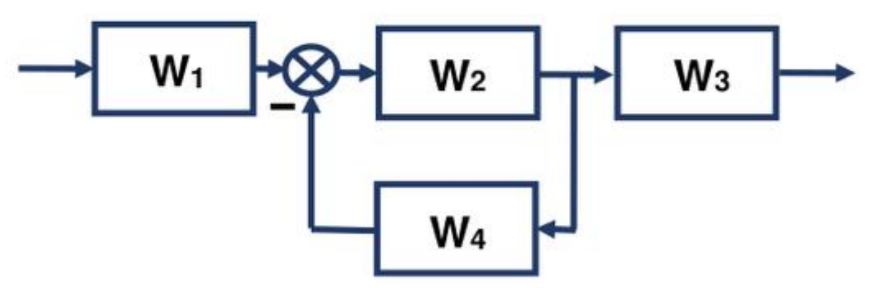
\includegraphics[width=0.9\textwidth]{sources/image2_1.png}
        \caption{Initial schema}
        \label{fig:plot1c}
\end{figure}
\subsection{Calculations}
Two blocks in the middle can be substituted with one with value $T= \frac{W_2}{1 + W_2 W_4}$. There is a plus in the denominator because the feedback is negative. Then the whole system is just three consecutive blocks, which can be transformed to one block with value equal to $W = \frac{W_1 W_2 W_3}{1 + W_2 W_4}$. Then we just substitute these transfer functions in this expression. So we get:
\begin{equation}W = 
	\frac{\frac{2}{s+5} \frac{s + 1}{s + 0.5} \frac{1}{s + 0.25}}
	{1 + \frac{s + 1}{s + 0.5} \frac{1}{2s + 3}} =
	\frac{2s^2 + 5s + 3}{s^4 + 7.75s^3 + 15.625s^2 + 9.6875s + 1.5625}
\end{equation}

\subsection{Simulink}
\begin{figure}[ht]
   	 \centering
     \begin{subfigure}[b]{0.47\textwidth}
         \centering
         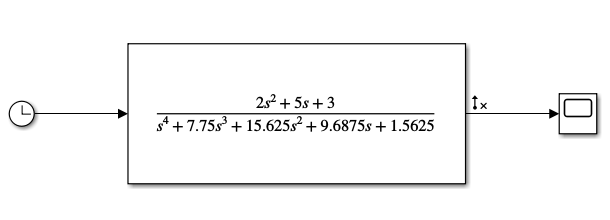
\includegraphics[width=\textwidth]{sources/image2_8.png}
         \caption{Original system}
         \label{fig:fig2}
     \end{subfigure}
     \hfill
     \begin{subfigure}[b]{0.47\textwidth}
         \centering
         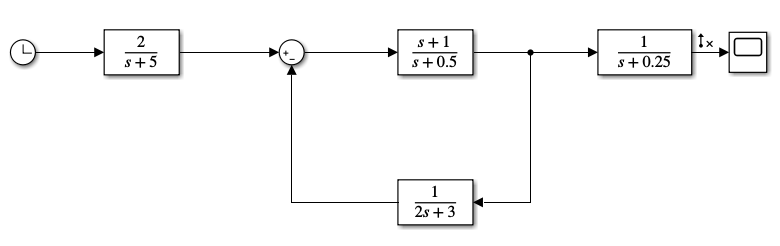
\includegraphics[width=\textwidth]{sources/image2_9.png}
         \caption{Simplified system}
         \label{fig:fig3}
     \end{subfigure}
     \caption{Simulink Schemas}
\end{figure}
Note that I change clock input to step block with step time 1 for step response; Pulse Generator with amplitude = 1000000000 (almost infinity), period = 100 sec, and pulse width 0.01 sec (almost small) for impulse response; Sin Wave block for frequency response. As you can see the systems are identical. It means that all calculations was correct.
\begin{figure}[ht]
   	 \centering
     \begin{subfigure}[b]{0.45\textwidth}
         \centering
         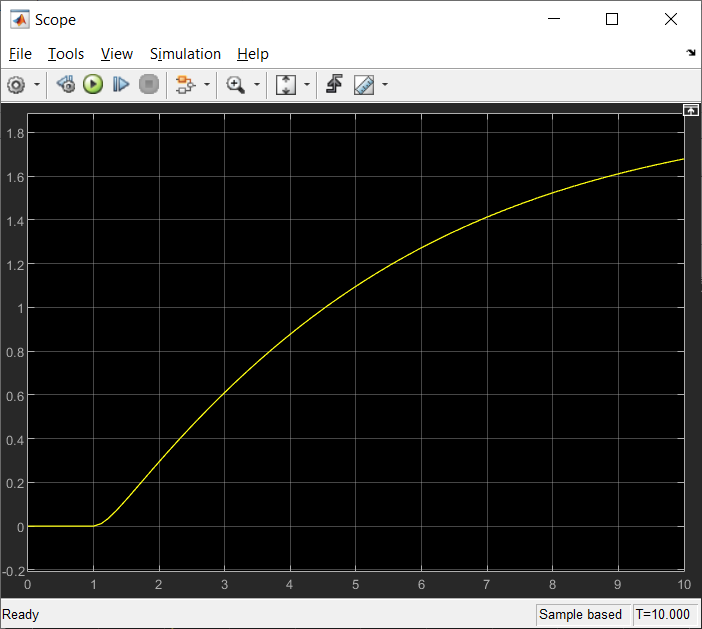
\includegraphics[width=\textwidth]{sources/image2_2.png}
         \caption{Original system}
         \label{fig:fig2}
     \end{subfigure}
     \hfill
     \begin{subfigure}[b]{0.45\textwidth}
         \centering
         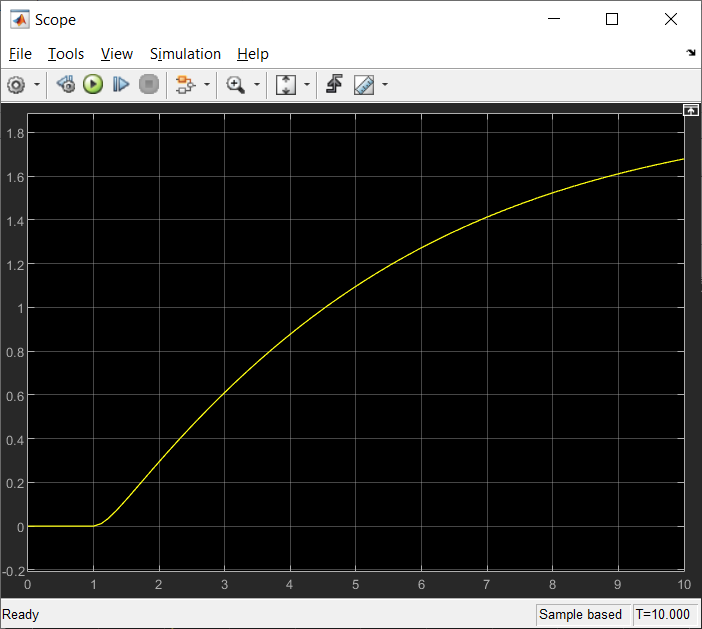
\includegraphics[width=\textwidth]{sources/image2_3.png}
         \caption{Simplified system}
         \label{fig:fig3}
     \end{subfigure}
     \caption{Step responses}
\end{figure}
\begin{figure}[ht]
   	 \centering
     \begin{subfigure}[b]{0.45\textwidth}
         \centering
         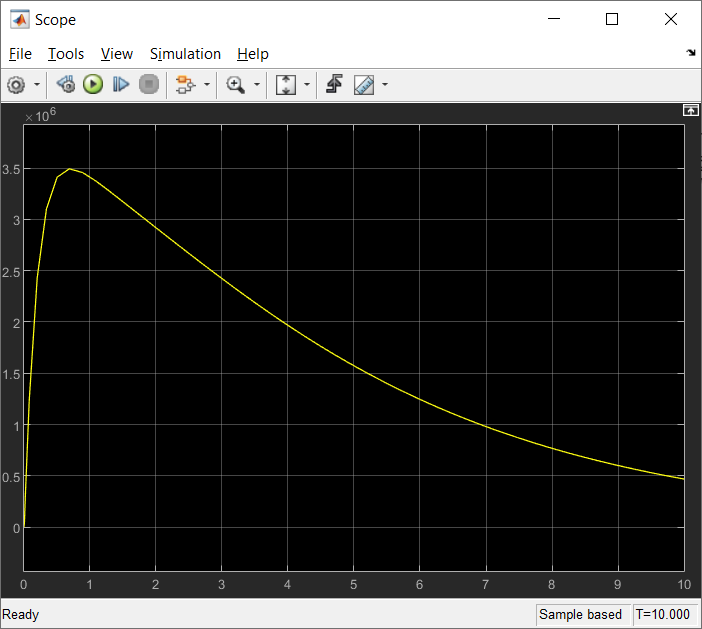
\includegraphics[width=\textwidth]{sources/image2_6.png}
         \caption{Original system}
         \label{fig:fig4}
     \end{subfigure}
     \hfill
     \begin{subfigure}[b]{0.45\textwidth}
         \centering
         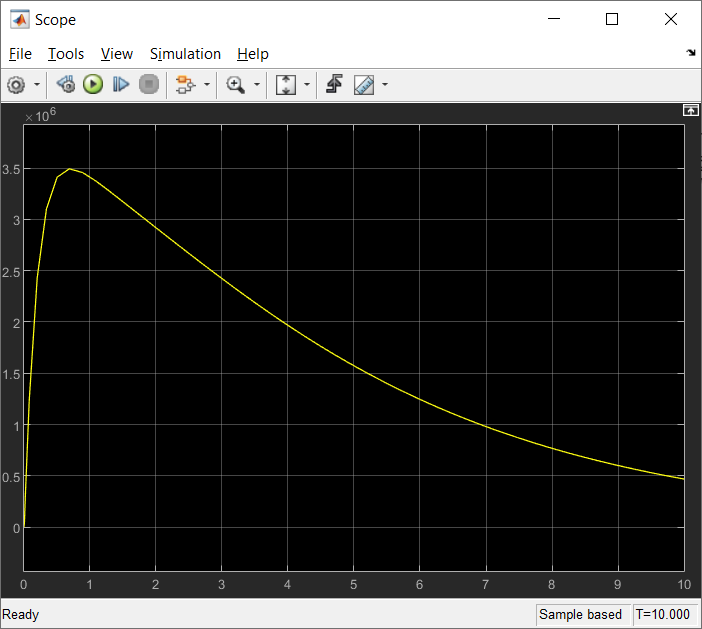
\includegraphics[width=\textwidth]{sources/image2_7.png}
         \caption{Simplified system}
         \label{fig:fig5}
     \end{subfigure}
     \caption{Impulse responses}
\end{figure}
\begin{figure}[H]
   	 \centering
     \begin{subfigure}[b]{0.45\textwidth}
         \centering
         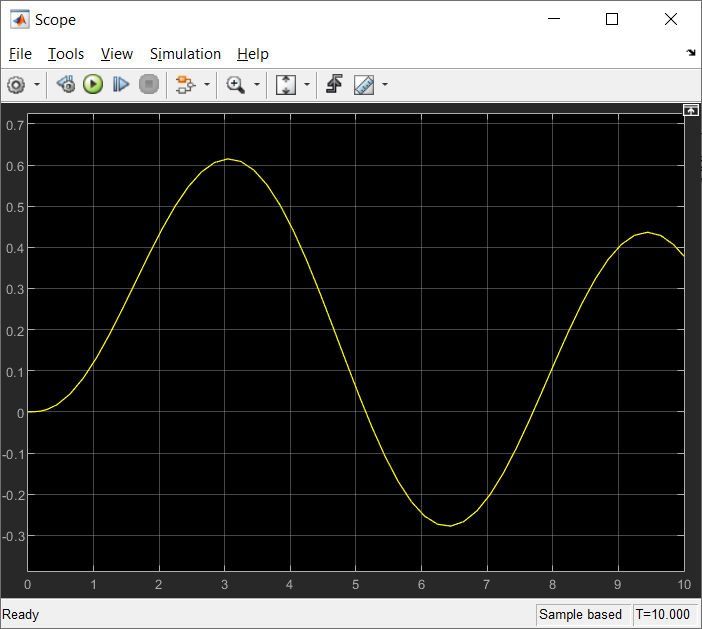
\includegraphics[width=\textwidth]{sources/image2_4.png}
         \caption{Original system}
         \label{fig:fig6}
     \end{subfigure}
     \hfill
     \begin{subfigure}[b]{0.45\textwidth}
         \centering
         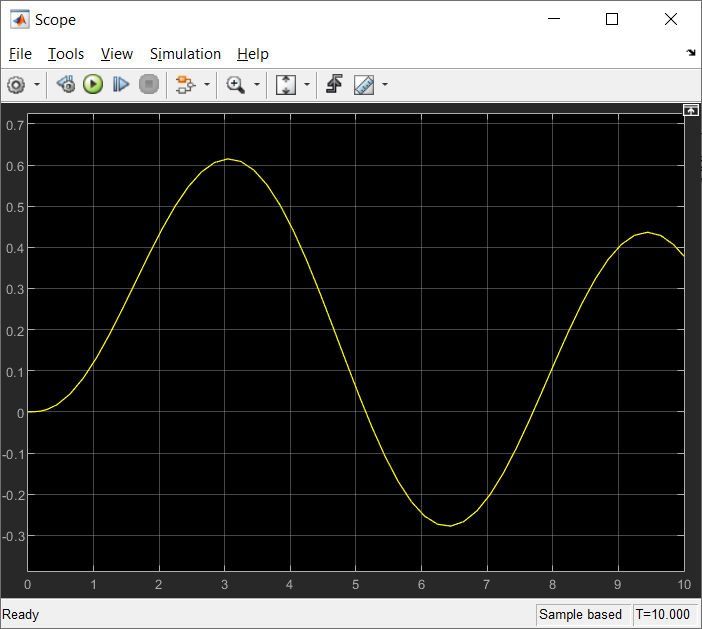
\includegraphics[width=\textwidth]{sources/image2_5.png}
         \caption{Simplified system}
         \label{fig:fig7}
     \end{subfigure}
     \caption{Frequency responses}
\end{figure}
\subsection{Bode and Pole-Zero plots}
I chose step input. 
\begin{figure}[H]
        \centering
        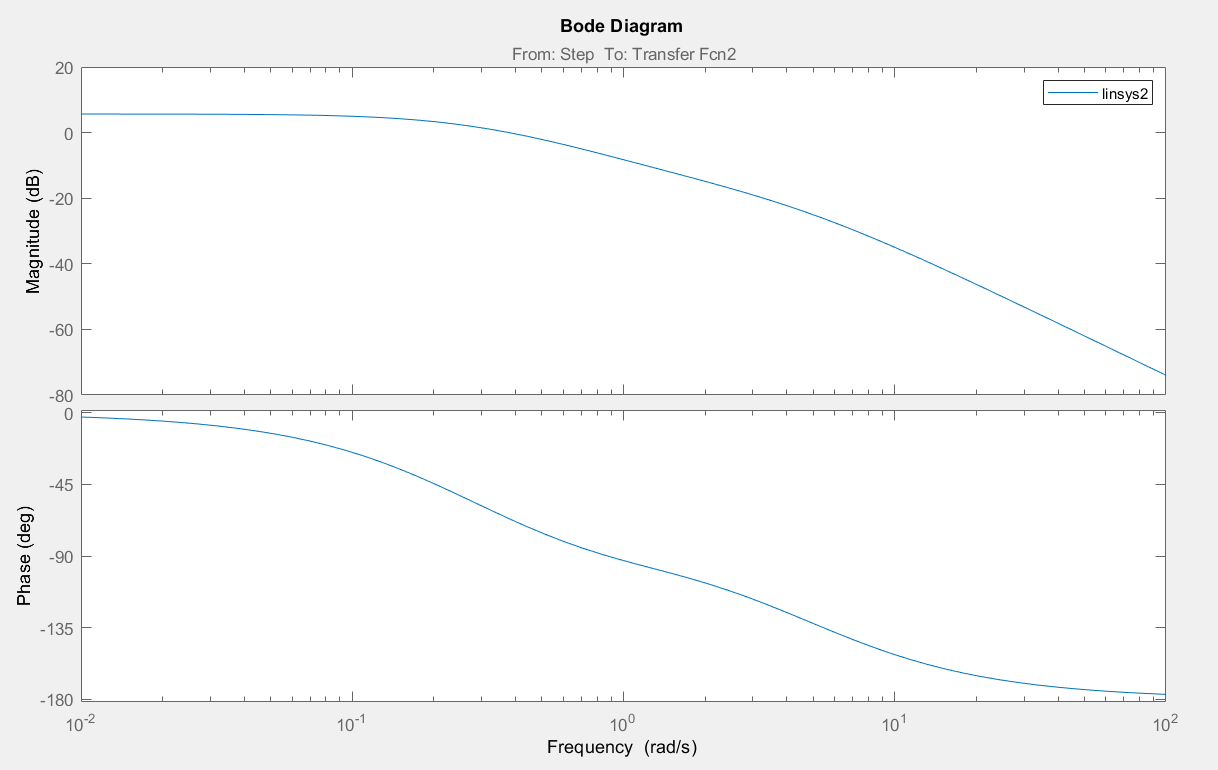
\includegraphics[width=0.9\textwidth]{sources/image2_10.png}
        \caption{Initial schema}
        \label{fig:bode1}
\end{figure}
The system is not stable since phase margin is less than gain margin.

\section{TTF}
\begin{figure}[H]
        \centering
        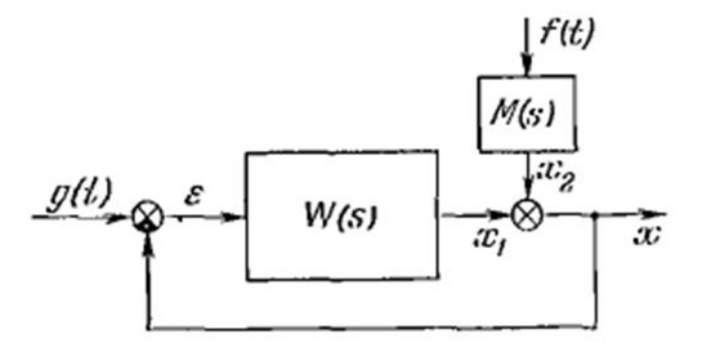
\includegraphics[width=0.9\textwidth]{sources/image3_1.png}
        \caption{The given system}
        \label{fig:bode1}
\end{figure}
In this case, the total transfer function is 
\begin{equation}
	T = \frac{W}{1+W}G + \frac{M}{1+W}F
\end{equation}
Let us just substitute the functions here:
\begin{equation}
	T = \frac{\frac{2}{s^2 + 2}}{1 + \frac{2}{s^2+2}} G + \frac{\frac{s + 2}{2s + 3}}{1 + \frac{2}{s^2 + 2}} F = 
	\frac{2}{s^2 + 4} G + \frac{s^3 + 2s^2 + 2s + 4}{2s^3 + 3s^2 + 8s + 12} F
\end{equation}
\section{SS2TF(1)}
In this task I used a formula that was given during one of the labs.
The transfer function can be calculated as followed:
\begin{equation}
	H = C (sI - A) ^{-1} B + D
\end{equation}
I wrote a program that evaluates this expression.
The program looks like:
\lstinputlisting[caption=Finding TF from the given SS in Matlab, label={lst:listing1}, language=Matlab]{sources/task4.m}
I got the following solution:
\begin{equation}
	H = \frac{s^2 - 3s - 8}{s ^ 2 - 5s + 8}
\end{equation}
\section{SS2TF(2)}
Using the same approach as I have used in the previous task I got:
\begin{align}
	T_1 &= \frac{s^2 - s - 18}{s^2 - 3s - 10}\\
	T_2 &= \frac{6s^2 - 13s - 68}{s^2 - 3s - 10}
\end{align}
The first one is transfer function for first input ($u_1$), the second one is for the second input ($u_2$).
Note that I used matrix approach that is general for any number of inputs and outputs. So, as a result we get a vector with all the transfer function we need.
\end{document}

